\documentclass{article}
\usepackage{mathtools}
\usepackage{amsmath}
\usepackage{amssymb}
\usepackage{tikz}
\usepackage{lipsum}
\usepackage{graphicx}
\usepackage[finnish]{babel}
\usepackage{fancyhdr}
\usepackage{pgf,tikz}


\pagestyle{fancy}

\newcounter{tehtava}
\setcounter{tehtava}{1}


\fancyhf{}
\fancyhead[L]{Tehtävä \thetehtava}

\fancypagestyle{plain}{
    \fancyhf{}
    \fancyhead[L]{Tehtävä \thetehtava}
}

\begin{document}
    \thispagestyle{plain}
	\title{MAT11001 - Harjoitus 5}
	\date{}
	\maketitle
	
	
	\section*{Tehtävä \thetehtava}
    Eräässä 150 henkilön ryhmässä 45 harrastaa uintia, 40 pyöräilyä ja 50 juoksua. Lisäksi 32
henkilöä harrastaa juoksua mutta ei pyöräilyä, 27 henkilöä harrastaa juoksua ja uintia ja 10
henkilöä harrastaa kaikkia kolmea lajia.

\paragraph*{}
Olkoon
\begin{itemize}
    \item $|J| = 50$ (50 henkilöä harrastaa juoksua)
    \item $|U| = 45$ (45 henkilöä harrastaa uintia)
    \item $|P| = 40$ (40 henkilöä harrastaa pyöräilyä)
    \item $|J \setminus P| = 32$  (juoksua mutta ei pyöräilyä)
    \item $|U \cap J| = 27$ (juoksua ja uintia)
    \item $|U \cap P \cap J| = 10$ (kaikkia kolmea lajia)
\end{itemize}



\paragraph*{}

\begin{itemize}
    \item[\textbf{a)}] Kuinka moni henkilöistä harrastaa juoksua mutta ei uintia eikä pyöräilyä?
    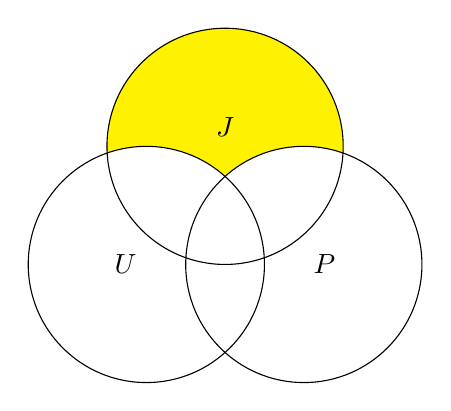
\begin{tikzpicture}
        % Määritellään ympyröiden keskipisteet ja säde
        \coordinate (U) at (-1,0); % Uinnin keskipiste
        \coordinate (P) at (1,0);  % Pyöräilyn keskipiste
        \coordinate (J) at (0,1.5);    % Juoksun keskipiste
        \def\R{1.5}                  % Ympyröiden säde
        
        % Varjostetaan alue J \ (U ∪ P)
        \begin{scope}
          \clip (J) circle (\R);             % Rajataan alue juoksun ympyrään
          \fill[yellow] (-4,-4) rectangle (4,4); % Täytetään koko alue keltaisella
          \fill[white] (U) circle (\R);      % Poistetaan uinnin ympyrän alue
          \fill[white] (P) circle (\R);      % Poistetaan pyöräilyn ympyrän alue
        \end{scope}
        
        % Piirretään ympyrät uudelleen, jotta reunat näkyvät selvästi
        \draw (U) circle (\R) node[left] {$U$};
        \draw (P) circle (\R) node[right] {$P$};
        \draw (J) circle (\R) node[above] {$J$};
        
        % Halutessasi voit lisätä alueiden numeeriset arvot tai merkinnät
        % Esimerkiksi:
        % \node at (-2,0) {$a$};
        % \node at (2,0) {$b$};
        % \node at (0,3) {$c$};
      \end{tikzpicture}
      Eli tarkoitus on löytää $|J \setminus (U \cup P)|$
      \begin{itemize}
        \item[1.] $|(J \cap U) \setminus P| = |U \cap J| - |U \cap P \cap J| = 27 - 10 = 17$
        \begin{itemize}
            \item $|U \cap J| = 27$ (kaikki juoksua harrastavat)
            \item $|U \cap P \cap J| = 10$ (harrastaa kaikkia lajeja)
            \item Vähentämällä saadaan ne henkilöit jotka harrastavat juoksua ja uintia mutta eivät pyöräilyä
        \end{itemize}
        \item[2.]Lasketaan ne henkilöt jotka harrastavat vain juoksua:
        \begin{itemize}
            \item $|J \setminus P| = 32$ (henkilöt jotka harrastavat juoksua mutta eivät pyöräilyä)
            \item Sijoitetaan tunnetut arvot: $32 = |J \setminus (U \cup P)| + 17$
            \item Ratkaistaan $|J \setminus (U \cup P)| \implies 32 - 17 = 15$
        \end{itemize}
        \item[3.]Vastaus:
        Juoksua mutta ei uintia eikä pyöräilyä harrastavien henkilöiden määrä on 15
      \end{itemize}
      

    \item[\textbf{b)}] Jos 21 henkilöä harrastaa sekä pyöräilyä että uintia, niin kuinka moni ei harrasta mitään kyseisistä kolmesta lajista?
    \begin{itemize}
        \item[\textbf{1.}] Lasketaan $|J \cap P|$ :\newline
        $|J \setminus P| = |J| - |J \cap P|$\newline
        Sijoitetaan tunnetut arvot: $32 = 50 - |J \cap P|$\newline  $\implies |J \cap P| = 50 - 32 = 18$
        \item[\textbf{2.}] Erotellaan kolmen joukon leikkaukset :
        \begin{itemize}
            \item kaikkia kolmea lajia harrastavat: $|U \cap P \cap J| = 10$
            \item sekä uintia että juoksua mutta eivät pyöräilyä harrastavat:\newline $|(U \cap J) \setminus P| = |U \cap J| - |U \cap P \cap J| = 27 - 10 = 17$
            \item sekä pyöräilyä että juoksua mutta eivät uintia harrastavat:\newline $|(P \cap J) \setminus U| = |P \cap J| - |U \cap P \cap J| = 18 - 10 = 8$
            \item sekä uintia että pyöräilyä mutta eivät juoksua harrastavat:\newline $|(U \cap P) \setminus J| = |U \cap P| - |U \cap P \cap J| = 21 - 10 = 11$
        \end{itemize}
        \item[\textbf{3.}] Lasketaan yksittäisten joukkojen vain omat osat:
        \begin{itemize}
            \item vain uinnin harrastajat:\newline $|U \setminus (P \cup J)| = |U| - |(U \cap P) \setminus J| - |(U \cap J) \setminus P| - |U \cap P \cap J| = 45 - 11 - 17 - 10 = 7$
            \item vain pyöräilyn harrastajat:\newline $|P \setminus (U \cup J)| = |P| - |(U \cap P) \setminus J| - |(P \cap J) \setminus U| - |U \cap P \cap J| = 40 - 11 - 8 - 10 = 11$
            \item Vain juoksun harrastajat:\newline$|J \setminus (U \cup P)| = 15$ (laskettiin kohdassa a)
        \end{itemize}
        \item[\textbf{4.}]Lasketaan kaikkien lajien harrastajien kokonaismäärä:
        \[
            \begin{aligned}
                N_{\text{harrastajat}} &= |U \setminus (P \cup J)| + |P \setminus (U \cup J)| + |J \setminus (U \cup P)| \\
                &+ |(U \cap P) \setminus J| + |(U \cap J) \setminus P| + |(P \cap J) \setminus U| \\
                &+ |U \cap P \cap J| \\
                &= 7 + 11 + 15 + 11 + 17 + 8 + 10 = 79
            \end{aligned}
        \]
        \item[\textbf{5.}]Henkilöt jotka eivät harrasta mitään näistä lajeista:\newline
        $\text{Kokonaismäärä} - N_{\text{harrastajat}} = 150 - 79 = 71$
    \end{itemize}
    Eli 71 henkilöä ei harrasta mitään näistä kolmesta lajista.
\end{itemize}


\newpage
\stepcounter{tehtava}
\section*{Tehtävä \thetehtava}

\end{document}